% !TeX root = ../main.tex

\chapter{龙芯安卓图形栈整体结构设计}
在实现安卓图形栈之前,需要对图形栈的运行机制从多个关键服务以及架构差异进行分析,并整理需要实现的模块及功能。

\section{图形栈系统分析}
\subsection{SurfaceFlinger关键服务分析}
Android图形系统作为移动端计算机的核心子系统,构建了从应用程序界面到物理显示设备的完整视觉呈现管道。
这个复杂的系统包含超过50个核心组件,其中SurfaceFlinger作为系统级的合成引擎,承担着最核心的图形处理任务。
整个系统的运作可以分解为三个层次架构:应用层、图形处理层和硬件抽象层。
应用层负责通过UI框架构建图形界面元素,图形处理层包括渲染引擎和合成器引擎,硬件抽象层主要是为这两个引擎提供支持。

渲染引擎分析:渲染引擎​是负责将抽象的图形描述转化为最终可视像素的软件系统。Android渲染引擎默认使用的是skia,
在SurfaceFlinger初始化过程中,会创建一个线程专门用于skia引擎的初始化并用于后续的图形绘制,
在SkiaGLRenderEngine::create时,会依次执行eglGetDisplay获取EGL显示句柄,此句柄代表了要渲染的物理设备;eglInitialize初始化EGL环境,并获得EGL的主次版本号;
eglQueryString查询与当前显示连接相关的字符串信息,包括EGL版本信息、供应商版本信息以及支持的客户端API等,安卓还会使用EGL\_EXTENSIONS
获取有关安卓特性的拓展并初始化;使用createEglContext在EGL中创建 OpenGL ES 上下文;然后使用eglMakeCurrent将指定的渲染上下文和表面设置为当前的函数。流程如图\ref{fig:skia_create过程}
因此渲染引擎的正常运行需要OpenGL ES相关实现支持。

\begin{figure}
  \centering
  \includegraphics[width=1\textwidth]{skia\_create过程.pdf}
  \caption{skia\_create过程}
  \label{fig:skia_create过程}
\end{figure}

合成器引擎分析:SurfaceFlinger中集成了合成器引擎CompositionEngine,也是SurfaceFlinger的核心部分,负责将多个图层按照z轴顺序合成并渲染等。
其作为硬件混合渲染器的客户端,会通过跨进程通信的方式调用框架中的Icomposer实现和接口,从而完成与具体硬件混合渲染器的交互。因此合成器引擎需要硬件混合渲染器实现的支持。
而合成器在合成图像时需要向系统申请图形缓存,因此也需要图形内存缓存分配的实现。

由上,为了实现对SurfaceFlinger的支持,需要OpengGL ES实现、硬件抽象层需要完成gralloc和HWC服务。 

\subsection{架构差异分析}
\label{sec:架构差异分析}
本课题需要在LoongArch架构下实现,而Android多应用于ARM架构,ARM与LoongArch架构的图形系统有较大差异,具体表现为ARM架构下的GPU没有独立显存\cite{Inki2011},
而在LoongArch的内核中,是使用DRI框架来调用GPU,并且GPU有自己的独立显存。
对LG110内存模型进行分析,LG110内存架构采用分层设计\ref{fig:LG110内存模型},包含GPU本地VRAM和系统主存中的GTT内存模块。
其实现原理体现为:GPU的VRAM通过PCI总线直接映射至CPU的地址空间,允许CPU通过标准PCIe协议直接访问这部分显存资源;
而GTT内存作为动态管理区域,借助页表机制将系统物理内存映射到虚拟地址空间,需经MMU转换后才能被访问。
就GPU端的数据访问逻辑而言,其采用分级的页表管理策略。针对本地VRAM区域,页表项直接记录该存储块的物理地址,使得GPU可直接基于物理地址进行存取操作;
而对于映射至系统主存的GTT区域,页表项存储的是经过DMA引擎转换后的设备地址,因此可以根据DMA的地址发起 DMA 请求获取数据。

\begin{figure}
  \centering
  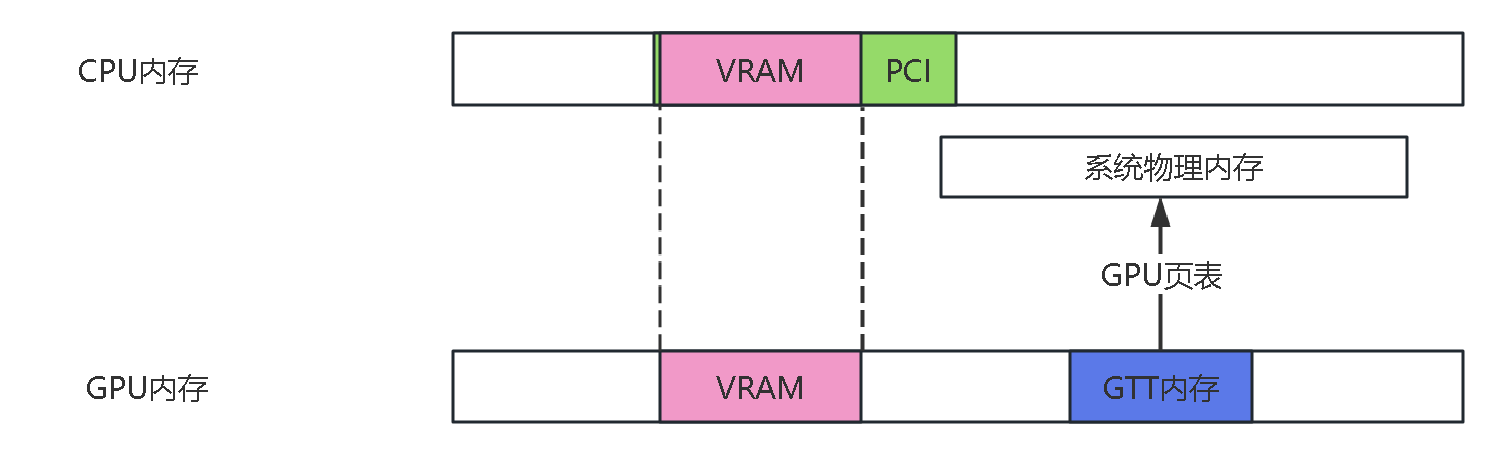
\includegraphics[width=0.8\textwidth]{LG110内存模型.pdf}
  \caption{LG110内存模型}
  \label{fig:LG110内存模型}
\end{figure}

因此,首先需要解决的是在LoongArch架构下,Android系统中显存和系统内存分配映射的问题。AndroidX86\cite{AndroidX86}
很大程度上解决这个问题,该项目使用Mesa作为OpenGL ES实现,基于DRM和GEM实现了gralloc模块,成功的在x86架构下运行SurfaceFlinger并实现硬件加速\cite{XTYY201710015}。
基于这个思路,我们也可以使用Mesa作为OpenGL ES实现以及mesa提供的GBM(General Buffer Manager)来管理缓冲区,
为此需要LoongArch架构的DRM框架和用户态libdrm的支持。其中DRM框架需要基于安卓通用内核5.10实现。

\subsection{安卓兼容性分析}
由于安卓是一个开源项目,因此任何硬件制造商都可以制造搭载安卓操作系统的设备,但兼容安卓的前提是可以正常运行安卓的执行环境和应用。
根据Android12的兼容性文档\cite{Android12CDD}中有关2D和3D图形加速的部分,对于显卡和配套驱动作出如下约束,必须支持OpenGL ES 1.1和2.0,
以及如下10种拓展\ref{tab:Android12兼容拓展要求}。目前龙芯LG110及配套已满足相关兼容性标准。

\begin{table}[h]
  \centering
  \caption{Android12兼容拓展要求}
  \label{tab:Android12兼容拓展要求}
  \begin{tabular}{l}
    \toprule
    拓展名  \\
    \midrule
    EGL\_KHR\_image \\
    EGL\_KHR\_image\_base \\
    EGL\_ANDROID\_image\_native\_buffer \\
    EGL\_ANDROID\_get\_native\_client\_buffer \\
    EGL\_KHR\_wait\_sync \\
    EGL\_KHR\_get\_all\_proc\_addresses \\
    EGL\_ANDROID\_presentation\_time \\
    EGL\_KHR\_swap\_buffers\_with\_damage \\
    EGL\_ANDROID\_recordable \\
    EGL\_ANDROID\_GLES\_layers \\
    \bottomrule
  \end{tabular}
  \note{}
\end{table}

\section{图形系统整体设计}
经过上节需求分析,课题为系统设计了基于龙芯显卡LG110的安卓图形系统方案。本节将对系统整体做一个概述。其中AOSP系统服务标注表示安卓系统服务部分,
loongson硬件支持标注表示现有的龙芯显卡实现相关的软件,需要部分适配,需实现部分标注表示需要实现的模块。

\begin{figure}[h]
  \centering
  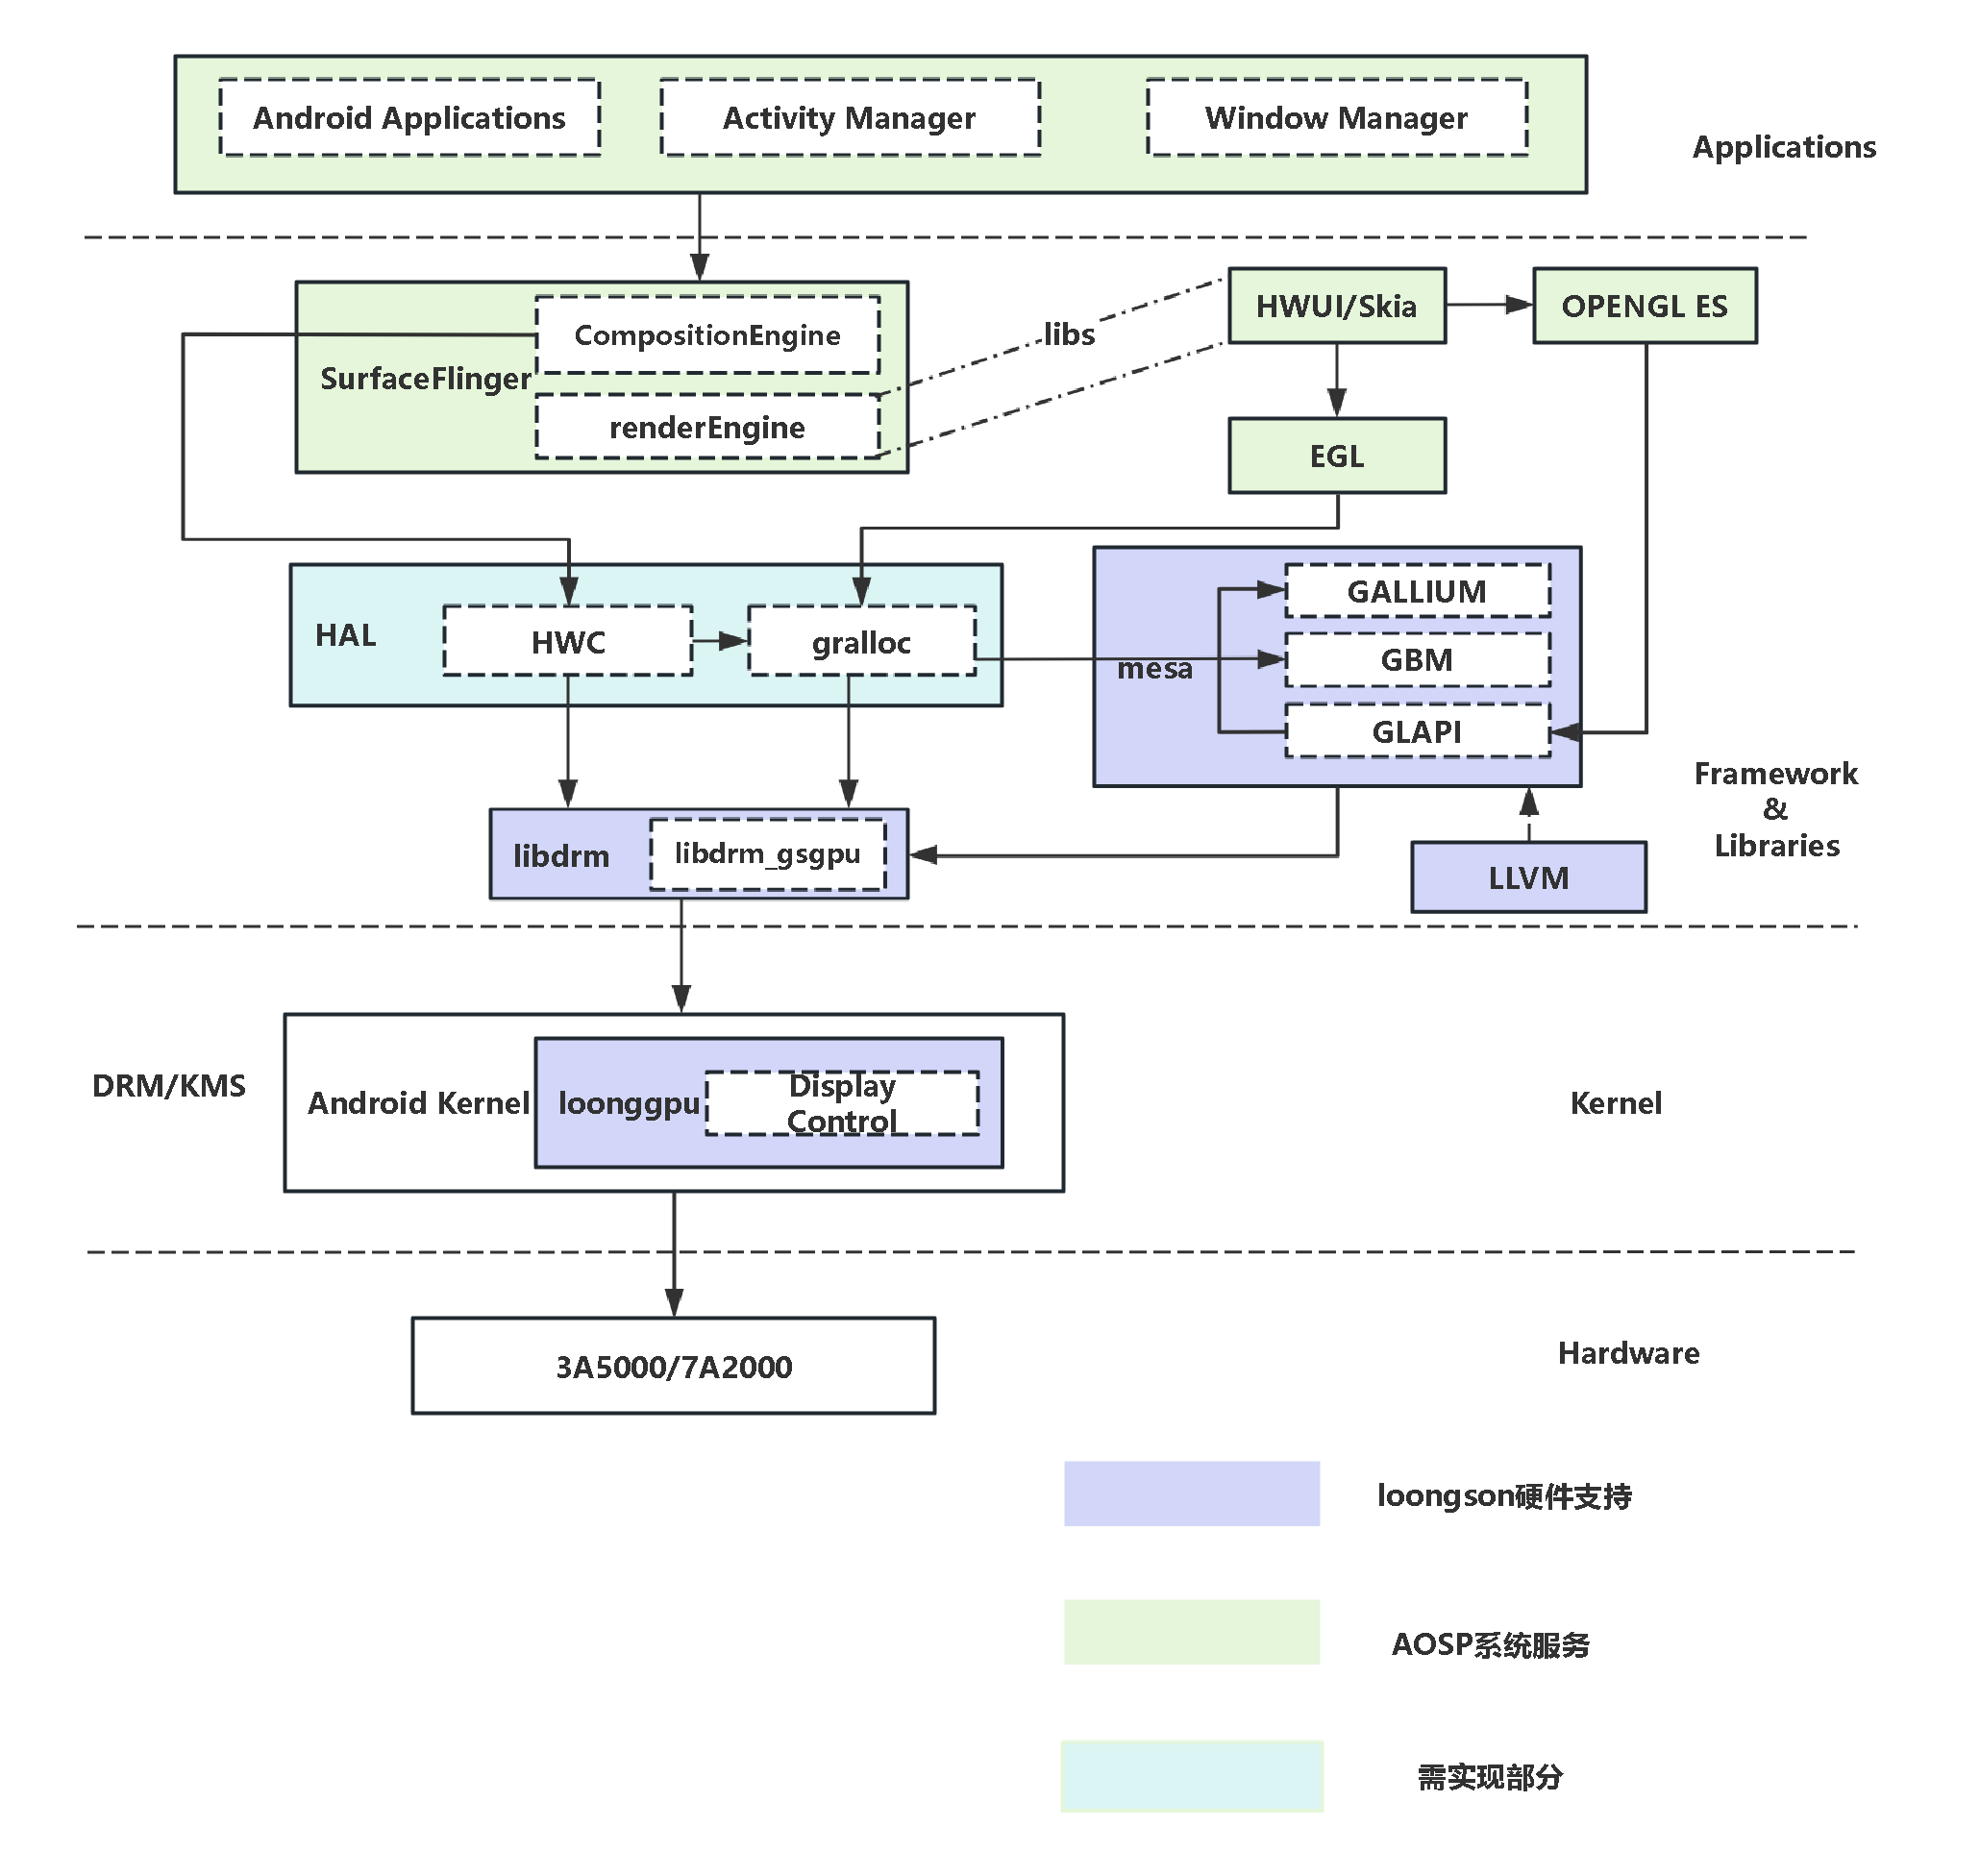
\includegraphics[width=1\textwidth]{图形栈总体结构图.pdf}
  \caption{图形栈总体结构图}    
  \label{fig:图形栈总体结构图}
\end{figure}

自上往下分析,Android应用(Android Applications)、活动管理器(Activity Manager)、窗口管理器(Window Manager)以及部分安卓Native程序(如BootAnimation)
等首先与Surface进行交互,根据自己的需求创建一个Surface,然后数个Surface会被SurfaceFlinger进行混合\cite{邓凡平2011深入理解}。
因此图形系统中最关键的服务进程就是SurfaceFlinger,负责管理图形缓冲区的合成与显示,如图\ref{fig:图形栈总体结构图}所示,它将来自不同应用的图形缓冲区进行合成,
并将合成结果发送到显示设备。SurafaceFlinger包含两个主要引擎合成引擎CompositionEngine和渲染引擎renderEngine,其中renderEngine在Android Q版本时被移至libs下作为相对独立的模块,
但仍然是SurfaceFlinger功能重要组成部分。CompositionEngine是作为HWC的客户端通过IPC方式调用HAL中HWC实现,而renderEngine主要是skia渲染引擎,该引擎通过EGL和OpenGL ES实现
3D硬件加速,需要HAL的gralloc和显卡OpenGL ES实现的支持。因此,图形系统的正确运行一个重要的环节就是确保SurfaceFlinger的正确运行。

而由上文可知,SurfaceFlinger的运行依赖于硬件抽象层和底层图形库。这其中有两个重要的模块,一个是HWC(硬件混合渲染器),是进行窗口合成和显示HAL层模块,其实现是特定于设备的,
通常是由显示设备制造商完成。其用于合成从Surfaceflinger接收的图层,从而减少GPU执行的合成量。
另一个模块是gralloc。它是Android中负责申请和释放GraphicBuffer的HAL层模块,
由硬件驱动提供实现,为BufferQueue机制提供了基础。gralloc的主要组件包括Allocator,Mapper。Allocator 负责内存的分配和释放,
主要功能包括:根据请求的大小和格式分配内存缓冲区,负责跟踪已分配和空闲的内存块以及支持在多个进程之间共享缓冲区,使得不同的应用程序或组件能够访问同一块内存。
Mapper负责将已分配的缓冲区映射到进程的虚拟地址空间。本课题需要实现支持龙芯硬件平台的gralloc和HWC模块的库以支持SurfaceFlinger的正确运行,即\ref{fig:图形栈总体结构图}中
需实现部分标注。

龙芯显卡驱动栈的方案,采用了mesa作为用户态驱动提供OpenGL ES实现和GBM加上DRM显示框架的方案。
安卓的framework层以及库函数依赖的图形接口是由libdrm进行封装,包括上文提及的gralloc和HWC都是需要使用libdrm定义的接口。
libdrm是一个用户态空间的库,提供了与 Linux 内核中的 DRM子系统交互的接口。它是 Linux 图形栈的核心组件之一(同样也是Android图形栈的方案),
通过封装 DRM 的 IOCTL 系统调用,为用户空间程序提供了简单易用的 API。
至于内核部分仍然是依赖linux内核的KMS和DRM。DRM/KMS 是 Linux 内核中用于管理图形硬件的子系统,提供了对 GPU、显示控制器和显示设备的统一抽象。在上层的系统级服务中,
SurfaceFlinger是通过HWC(Hardware Composer)与DRM/KMS交互,HWC负责将图形缓冲区合成任务委托给硬件。在 DRM/KMS 框架下,HWC 通过 DRM 接口与内核通信,
管理显示模式设置、缓冲区分配和显示同步等任务。KMS 负责配置显示控制器和显示设备的分辨率、刷新率等参数,而 DRM 则管理图形缓冲区的分配与渲染。
OpenGL ES的实现是由用户态驱动mesa提供,而mesa实现的OpenGL ES接口在已有的X图形协议上已有过相关测试。

%在后续章节中,将从驱动内核模块、用户态驱动、Android HAL层实现以及系统镜像定制等4个部分说明方案。

\section{系统需求分析}

由上节关键服务分析可知,需要在安卓硬件抽象层实现gralloc和HWC服务。安卓系统较为特殊,其本身对于模块的实现有着严格的接口定义和规范。
自Android Q版本开始,为了提供图形性能和增强对硬件的支持,对图形系统进行了重构与优化,至S版本稳定下来,中间迭代了4个API版本,
具体表现为,引入了Gralloc2 API(至Android S版本Gralloc4稳定)和HWC2,本课题基于gralloc4以及composer2.1实现。
gralloc模块需要完成内存分配、缓冲区映射、缓冲区管理、性能优化等多方面的功能,hwcomposer模块则需要实现图层管理、显示输出、合成控制、与gralloc适应相关的功能。
gralloc模块HAL接口分别定义在/hardware/interfaces/graphics/allocator和/hardware/interfaces/graphics/mapper下,
其中HAL接口表统计如表\ref{tab:gralloc模块HAL接口}。
而HWC模块的实现较为复杂,包含服务端和客户端,服务端的实现集中在/hardware/interfaces/graphics/composer下,
服务端钟具体EGL的调用是由硬件供应商实现并通过私有调用回安卓合成系统用于最终的缓冲区显示\cite{baiget2019architecture},
客户端是指如SurfaceFlinger中的CompositionEngine通过跨进程调用服务端的实现。

\begin{table}[h]
  \centering
  \caption{gralloc模块HAL接口}
  \label{tab:gralloc模块HAL接口}
  \begin{tabular}{llll}
    \toprule
    接口  & 组 & 接口 & 组\\
    \midrule
    createDescriptor & IMapper & get & IMapper \\
    importBuffer & IMapper & set & IMapper\\
    freeBuffer & IMapper & getFromBufferDescriptorInfo & IMapper\\
    validateBufferSize & IMapper & listSupportedMetadataTypes & IMapper\\
    getTransportSize & IMapper & dumpBuffer  & IMapper\\
    lock & IMapper & getReservedRegion & IMapper\\
    unlock & IIMapper & allocate & IAllocator\\
    flushLockedBuffer & IMapper & isSupported & IMapper\\
    rereadLockedBuffer & IMapper \\
    \bottomrule
  \end{tabular}
  \note{}
\end{table}

\subsection{图形缓存分配模块需求分析}

\subsubsection{功能需求}

    ​GPU硬件兼容性​:支持GSGPU等LoongArch下GPU驱动。适配DRM/KMS接口,正确处理IOCTL命令。

    ​缓冲区分配与管理​:支持常见像素格式及修饰符。实现显存与系统内存的自动选择策略,优先使用显存提升性能。

    ​跨API共享​:通过DMA机制导出缓冲区句柄,支持跨进程间的零拷贝数据传输。提供缓冲区对象的导入/映射接口,兼容EGL/GLES纹理绑定流程。

\subsubsection{性能优化}

    ​内存复用​​:设计缓冲区缓存池,减少频繁分配/释放带来的内存碎片及性能开销。

    ​异步操作支持​:提供异步缓冲区映射接口,避免阻塞渲染线程。

\subsubsection{非功能需求}
        
    兼容性:兼容Android 12,支持Kernel 5.10及DRM/KMS子系统。
        
    安全性:​确保不同进程的缓冲区访问权限隔离以实现内存隔离,缓冲区对象需通过引用计数自动释放以抗内存泄漏

    可维护性:分离硬件后端与通用逻辑,便于新增GPU支持,集成Android Logcat,提供关键操作的调试日志。

\subsection{硬件混合渲染模块需求分析}

\subsubsection{功能需求}

显示管道管理​:支持通过 libdrm 接口与内核 DRM 子系统交互,通过KMS(Kernel Mode Setting)设置分辨率、刷新率,支持热插拔检测与模式切换,支持原子更新,
支持同时管理多个Connector,动态创建/销毁DRM显示管道实例。

​图层混合与合成​:支持硬件混合与回退到 GPU 合成。支持基础图层(Primary)、叠加图层(Overlay)、光标(Cursor)等类型,
需适配DRM Plane类型(DRM\_PLANE\_TYPE\_PRIMARY/OVERLAY/CURSOR),支持缩放、旋转、透明度混合、裁剪区域设置。

​缓冲区管理​:基于Gralloc的缓冲区管理,将应用程序生成的图像资源统一转化为显示控制器可识别的标准化帧结构。

\subsubsection{非功能需求}

​兼容性​:适配主流 DRM 系统,支持龙芯LG系列GPU的显存管理,兼容 Android 10+的HIDL接口。

稳定性与安全性:支持 DRM Master 丢失后重新初始化显示管道以实现异常恢复,单个Connector故障不影响其他显示输出

\section{本章小结}
本章围绕着安卓图形栈的运行机制进行分析,并对整体结构进行了描述,并对两个主要模块,图形缓存分配模块和硬件混合渲染模块的需求进行分析。

